\documentclass[handout]{beamer}
\setbeamertemplate{footline}[frame number]
%\documentclass{beamer}

\usepackage[utf8x]{inputenc}
\usepackage[brazil,british]{babel}
\usetheme{default} 
\usecolortheme{beaver}
\newtranslation[to=brazil]{Theorem}{Teorema}
\newtranslation[to=brazil]{Definition}{Definição}
\newtranslation[to=brazil]{Example}{Exemplo}
\newtranslation[to=brazil]{Problem}{Exercício}
\newtranslation[to=brazil]{Solution}{Resolução}
\logo{
\includegraphics[width=1cm]{../img/logo-ppgsc-icon-text.png}}

\usepackage{graphicx}
\usepackage{clrscode3e}
\usepackage{hyperref}

\usepackage{pgf}
\usepackage{tikz}
\newcommand{\assert}[1]{\textcolor{blue}{#1}}



\usepackage{pgf}
\usepackage{tikz}

\title{Aula 06: Análise matemática de algoritmos recursivos}
\author{David Déharbe \\
  Programa de Pós-graduação em Sistemas e Computação \\
  Universidade Federal do Rio Grande do Norte \\
  Centro de Ciências Exatas e da Terra \\
  Departamento de Informática e Matemática Aplicada}
\date{}

\begin{document}
\selectlanguage{brazil}
\begin{frame}
  \titlepage
\end{frame}

\section{Introdução}

\begin{frame}

  \frametitle{Contexto}

  \begin{center}
  \begin{pgfpicture}{0cm}{0cm}{9cm}{7.3cm}
  \pgfsetendarrow{\pgfarrowtriangle{3pt}}

  \pgfrect[stroke]{\pgfxy(2,6.5)}{\pgfxy(5,.8)}
  \pgfputat{\pgfxy(4.5,6.9)}{\pgfbox[center,center]{Entender problema}}
  \pgfline{\pgfxy(4.5,6.5)}{\pgfxy(4.5,6.0)}

  \pgfrect[stroke]{\pgfxy(2,5.2)}{\pgfxy(5,.8)}
  \pgfputat{\pgfxy(4.5,5.6)}{\pgfbox[center,center]{Escolher abordagem}}
  \pgfline{\pgfxy(4.5,5.2)}{\pgfxy(4.5,4.7)}

  \pgfrect[stroke]{\pgfxy(2,3.9)}{\pgfxy(5,.8)}
  \pgfputat{\pgfxy(4.5,4.3)}{\pgfbox[center,center]{Projetar algoritmo}}
  \pgfline{\pgfxy(4.5,3.9)}{\pgfxy(4.5,3.4)}

  \pgfrect[stroke]{\pgfxy(2,2.6)}{\pgfxy(5,.8)}
  \pgfputat{\pgfxy(4.5,3.0)}{\pgfbox[center,center]{Provar correção}}
  \pgfline{\pgfxy(4.5,2.6)}{\pgfxy(4.5,2.1)}
  \pgfmoveto{\pgfxy(2.0,3.0)}
  \pgfcurveto{\pgfxy(1.5,3.0)}{\pgfxy(1.5,4.3)}{\pgfxy(2.0,4.3)}
  \pgfstroke
  \pgfmoveto{\pgfxy(2.0,3.0)}
  \pgfcurveto{\pgfxy(1.0,3.0)}{\pgfxy(1.0,5.6)}{\pgfxy(2.0,5.6)}
  \pgfstroke

  \pgfsetcolor{lightgray}
  \pgfrect[fill]{\pgfxy(2,1.3)}{\pgfxy(5,.8)}
  \pgfsetcolor{black}
  \pgfputat{\pgfxy(4.5,1.7)}{\pgfbox[center,center]{Analizar complexidade}}
  \pgfline{\pgfxy(4.5,1.3)}{\pgfxy(4.5,0.8)}
  \pgfmoveto{\pgfxy(7.0,1.7)}
  \pgfcurveto{\pgfxy(7.5,1.7)}{\pgfxy(7.5,4.3)}{\pgfxy(7.0,4.3)}
  \pgfstroke
  \pgfmoveto{\pgfxy(7.0,1.7)}
  \pgfcurveto{\pgfxy(8.0,1.7)}{\pgfxy(8.0,5.6)}{\pgfxy(7.0,5.6)}
  \pgfstroke

  \pgfrect[stroke]{\pgfxy(2,0)}{\pgfxy(5,.8)}
  \pgfputat{\pgfxy(4.5,0.4)}{\pgfbox[center,center]{Codificar algoritmo}}
\end{pgfpicture}
  \end{center}
\end{frame}


\begin{frame}

  \frametitle{Estrutura da apresentação}

  \begin{description}
  \item[1] arcabouço teórico;
  \item[2] melhor caso, pior caso, caso médio;
  \item[3] notações asintóticas; $O$, $\Omega$, $\Theta$;
  \item[4] análise de algoritmos não recursivos;
  \item[5] \alert{análise de algoritmos recursivos}.
  \end{description}
\end{frame}

\begin{frame}

  \frametitle{Bibliografia usada}

  \begin{center}
    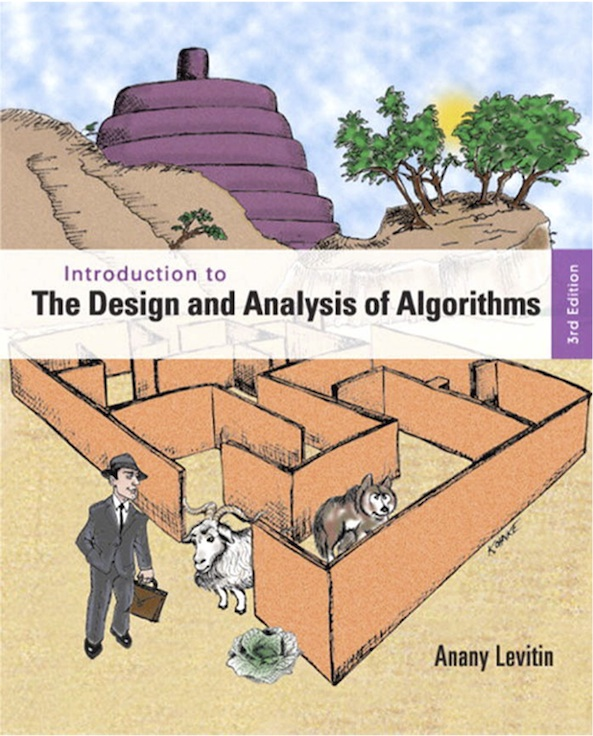
\includegraphics[height=.8\textheight]{img/capa-levitin.jpg}
  \end{center}
  (seções 2.4, 2.5)
\end{frame}

\section{Um exemplo introdutório}

\begin{frame}
  \frametitle{Exemplo introdutório}

  \begin{example}[Fatorial]
    \begin{codebox}
\Procname{$\proc{F}(n)$}
\li \If $n = 0$ \kw{then} \Return $1$
\li \Else \Return $n \times F(n-1)$
\end{codebox}

  \end{example}
  \pause

\begin{itemize}
\item Tamanho da entrada: $n$.
\item Operação básica: \alert{multiplicação}/teste $n=0$/chamada recursiva
\item Seja $M(n)$ o número de multiplicações:
\begin{itemize}
\item $M(n) = 1 + M(n-1)$
\item $M(0) = 0$
\end{itemize}
\item $M$ é definida por recorrência. Como encontrar uma expressão fechada,
não recursiva, de $M(n)$?
\end{itemize}
\end{frame}

\begin{frame}
  \frametitle{Plano da aula}
  \tableofcontents
\end{frame}

\begin{frame}
  \frametitle{Resolução de recorrência por substituição}

\begin{eqnarray*}
M(n) & = & 1 + M(n-1) \\
& = & 1 + (1 + M(n-2)) = 2 + M(n-2) \\
& = & 2 + (1 + M(n-3)) = 3 + M(n-3) 
\end{eqnarray*}
\begin{itemize}
\item Conjectura: $M(n) = i + M(n-i)$
\item Como é conhecido $M(0) = 0 = M(n-n)$, então $M(n) = n + M(0) = n$.
\end{itemize}
\end{frame}

\section{Estratégia de análise}

\begin{frame}
\frametitle{Estratégia de análise}
\begin{enumerate}
\item Identificar um parâmetro representando o tamanho da entrada
\item Identificar a operação básica do algoritmo
\item Verificar se o número de vezes que a operação básica é executada pode
  variar com entradas do mesmo tamanho.

  Se for o caso, o pior caso, a complexidade média e o melhor caso devem ser
  averiguados individualmente.
\item Estabelecer uma relação de recorrência que corresponde ao número de vezes que uma operação é executada. Estabelecer o valor inicial também.

\item Resolver a recorrência. Pelo menos, enquadrar o crescimento asintótico da
  relação.
\end{enumerate}
\end{frame}

\section{Exemplo 2}
\begin{frame}
\frametitle{Torres de Hanoi}

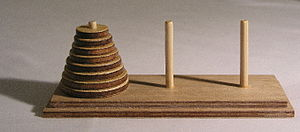
\includegraphics{../img/hanoi.jpeg}

A Torre de Hanói é um "quebra-cabeça" que consiste em uma base contendo três
pinos, em um dos quais são dispostos alguns discos uns sobre os outros, em ordem
crescente de diâmetro, de cima para baixo. O problema consiste em passar todos
os discos de um pino para outro qualquer, usando um dos pinos como auxiliar, de
maneira que um disco maior nunca fique em cima de outro menor em nenhuma
situação.  (Wikipedia)

\end{frame}

\begin{frame}
\frametitle{Resolução (recursiva)}

\begin{codebox}
\Procname{$\proc{Hanoi}(n, \id{src}, \id{dest}, \id{aux})$} 
\li \If $n = 1$
\li \Then
    \Return $\proc{Move}(\id{src}, \id{dest})$
\li \Else
\li   $\proc{Hanoi}(n-1, \id{src}, \id{aux}, \id{dest})$
\li   $\proc{Move}(\id{src}, \id{dest})$
\li   $\proc{Hanoi}(n-1, \id{aux}, \id{dest}, \id{src})$
    \End
\end{codebox}


\end{frame}

\begin{frame}
\frametitle{Aplicação da estratégia}

\begin{small}
\begin{codebox}
\Procname{$\proc{Hanoi}(n, \id{src}, \id{dest}, \id{aux})$} 
\li \If $n = 1$
\li \Then
    \Return $\proc{Move}(\id{src}, \id{dest})$
\li \Else
\li   $\proc{Hanoi}(n-1, \id{src}, \id{aux}, \id{dest})$
\li   $\proc{Move}(\id{src}, \id{dest})$
\li   $\proc{Hanoi}(n-1, \id{aux}, \id{dest}, \id{src})$
    \End
\end{codebox}

\end{small}
\begin{itemize}
\item Tamanho da entrada: $n$
\item Operação básica: mover um disco
\item $M(n) = M(n-1) + 1 + M(n-1) = 2 \times M(n-1) + 1$ se $n > 1$
\item $M(1) = 1$.
\item Resolver $M$.
\end{itemize}
\end{frame}

\begin{frame}
\frametitle{Aplicação da estratégia}

\begin{eqnarray*}
M(n) & = & 2 \times M(n-1) + 1 \pause \\
     & = & 2 \times (2 \times M(n-2) + 1) + 1 \pause = 4 \times M(n-2) + 3 \pause \\
     & = & 4 \times (2 \times M(n-3) + 1) + 3 \pause = 8 \times M(n-3) + 7 \pause \\
     & \cdots & \\
     & = & 2^i \times M(n-i) + (2^i - 1) \pause \\
     & \cdots & \mbox{(note que $1 = n - (n - 1)$)}\\
     & = & 2^{n-1} \times M(n-(n-1)) + (2^{n-1} - 1) \pause \\
     & = & 2^{n-1} \times M(1) + 2^{n-1} - 1 \pause \\
     & = & 2^{n-1} + 2^{n-1} - 1 \pause \\
     & = & 2 \times 2^{n-1} - 1 \pause \\
\alert{M(n)} & \alert{=} & \alert{2^n - 1}
\end{eqnarray*}

\end{frame}

\begin{frame}
\frametitle{Observações}
\begin{itemize}
\item A resolução recursiva do problema das Torres de Hanoi cabe em 5 linhas.
\item Tem complexidade exponencial
\item No caso, não tem solução mais eficiente.
\item Mas cuidado: concisão não é sinônimo de eficiência!
\end{itemize}
\end{frame}

\begin{frame}
\frametitle{Árvore das chamadas recursivas}
Permite visualizar todas as chamadas realizadas por um algoritmo recursivo: pode ser útil para analizar a complexidade.

\begin{center}
\begin{pgfpicture}{0cm}{0cm}{12cm}{5cm}
  \pgfputat{\pgfxy(0, .5)}{\pgfbox[center,center]{1}}
  \pgfputat{\pgfxy(1, .5)}{\pgfbox[center,center]{1}}
  \pgfputat{\pgfxy(2, .5)}{\pgfbox[center,center]{1}}
  \pgfputat{\pgfxy(3, .5)}{\pgfbox[center,center]{1}}
  \pgfputat{\pgfxy(8, .5)}{\pgfbox[center,center]{1}}
  \pgfputat{\pgfxy(9, .5)}{\pgfbox[center,center]{1}}
  \pgfputat{\pgfxy(10, .5)}{\pgfbox[center,center]{1}}
  \pgfputat{\pgfxy(11, .5)}{\pgfbox[center,center]{1}}

  \pgfputat{\pgfxy(0.5, 1.5)}{\pgfbox[center,center]{2}}
  \pgfxyline(0.4,1.4)(0.1,0.6)
  \pgfxyline(0.6,1.4)(0.9,0.6)
  \pgfputat{\pgfxy(2.5, 1.5)}{\pgfbox[center,center]{2}}
  \pgfxyline(2.4,1.4)(2.1,0.6)
  \pgfxyline(2.6,1.4)(2.9,0.6)
  \pgfputat{\pgfxy(8.5, 1.5)}{\pgfbox[center,center]{2}}
  \pgfxyline(8.4,1.4)(8.1,0.6)
  \pgfxyline(8.6,1.4)(8.9,0.6)
  \pgfputat{\pgfxy(10.5, 1.5)}{\pgfbox[center,center]{2}}
  \pgfxyline(10.4,1.4)(10.1,0.6)
  \pgfxyline(10.6,1.4)(10.9,0.6)

  \pgfputat{\pgfxy(2, 2)}{\pgfbox[center,center]{$\cdots$}}
  \pgfputat{\pgfxy(4, 2)}{\pgfbox[center,center]{$\cdots$}}
  \pgfputat{\pgfxy(10, 2)}{\pgfbox[center,center]{$\cdots$}}

  \pgfputat{\pgfxy(2, 2.5)}{\pgfbox[center,center]{$n-2$}}
  \pgfputat{\pgfxy(4, 2.5)}{\pgfbox[center,center]{$n-2$}}
  \pgfputat{\pgfxy(7, 2.5)}{\pgfbox[center,center]{$n-2$}}
  \pgfputat{\pgfxy(9, 2.5)}{\pgfbox[center,center]{$n-2$}}

  \pgfputat{\pgfxy(3, 3.5)}{\pgfbox[center,center]{$n-1$}}
  \pgfxyline(2.9,3.4)(2.1,2.6)
  \pgfxyline(3.1,3.4)(3.9,2.6)
  \pgfputat{\pgfxy(8, 3.5)}{\pgfbox[center,center]{$n-1$}}
  \pgfxyline(7.9,3.4)(7.1,2.6)
  \pgfxyline(8.1,3.4)(8.9,2.6)

  \pgfputat{\pgfxy(5.5, 4.5)}{\pgfbox[center,center]{$n$}}
  \pgfxyline(5.4,4.4)(3.1,3.6)
  \pgfxyline(5.6,4.4)(7.9,3.6)

  \pgfsetendarrow{\pgfarrowtriangle{3pt}}
%   \pgfrect[stroke]{\pgfxy(2,6.5)}{\pgfxy(5,.8)}
%   \pgfputat{\pgfxy(4.5,6.9)}{\pgfbox[center,center]{Entender problema}}
%   \pgfline{\pgfxy(4.5,6.5)}{\pgfxy(4.5,6.0)}

%   \pgfrect[stroke]{\pgfxy(2,5.2)}{\pgfxy(5,.8)}
%   \pgfputat{\pgfxy(4.5,5.6)}{\pgfbox[center,center]{Escolher abordagem}}
%   \pgfline{\pgfxy(4.5,5.2)}{\pgfxy(4.5,4.7)}

%   \pgfrect[stroke]{\pgfxy(2,3.9)}{\pgfxy(5,.8)}
%   \pgfputat{\pgfxy(4.5,4.3)}{\pgfbox[center,center]{Projetar algoritmo}}
%   \pgfline{\pgfxy(4.5,3.9)}{\pgfxy(4.5,3.4)}

%   \pgfrect[stroke]{\pgfxy(2,2.6)}{\pgfxy(5,.8)}
%   \pgfputat{\pgfxy(4.5,3.0)}{\pgfbox[center,center]{Provar correção}}
%   \pgfline{\pgfxy(4.5,2.6)}{\pgfxy(4.5,2.1)}
%   \pgfmoveto{\pgfxy(2.0,3.0)}
%   \pgfcurveto{\pgfxy(1.5,3.0)}{\pgfxy(1.5,4.3)}{\pgfxy(2.0,4.3)}
%   \pgfstroke
%   \pgfmoveto{\pgfxy(2.0,3.0)}
%   \pgfcurveto{\pgfxy(1.0,3.0)}{\pgfxy(1.0,5.6)}{\pgfxy(2.0,5.6)}
%   \pgfstroke

%   \pgfsetcolor{lightgray}
%   \pgfrect[fill]{\pgfxy(2,1.3)}{\pgfxy(5,.8)}
%   \pgfsetcolor{black}
%   \pgfputat{\pgfxy(4.5,1.7)}{\pgfbox[center,center]{Analizar complexidade}}
%   \pgfline{\pgfxy(4.5,1.3)}{\pgfxy(4.5,0.8)}
%   \pgfmoveto{\pgfxy(7.0,1.7)}
%   \pgfcurveto{\pgfxy(7.5,1.7)}{\pgfxy(7.5,4.3)}{\pgfxy(7.0,4.3)}
%   \pgfstroke
%   \pgfmoveto{\pgfxy(7.0,1.7)}
%   \pgfcurveto{\pgfxy(8.0,1.7)}{\pgfxy(8.0,5.6)}{\pgfxy(7.0,5.6)}
%   \pgfstroke

%   \pgfrect[stroke]{\pgfxy(2,0)}{\pgfxy(5,.8)}
%   \pgfputat{\pgfxy(4.5,0.4)}{\pgfbox[center,center]{Codificar algoritmo}}
\end{pgfpicture}
\end{center}

\end{frame}


\section{Exemplo 3}
\begin{frame}
\frametitle{Número de algarismos binários de um inteiro}

\begin{codebox}
\Procname{$\proc{Binary}(n$)} 
\li \If $n \le 1$
\li \Then
      \Return $1$
\li \Else
\li   \Return $\proc{Binary}(\lfloor n/2 \rfloor)$ + 1
    \End
\end{codebox}


\end{frame}

\begin{frame}
\frametitle{Aplicação da estratégia}
\begin{small}
\begin{codebox}
\Procname{$\proc{Binary}(n$)} 
\li \If $n \le 1$
\li \Then
      \Return $1$
\li \Else
\li   \Return $\proc{Binary}(\lfloor n/2 \rfloor)$ + 1
    \End
\end{codebox}

\end{small}
\begin{itemize}
\item Tamanho da entrada: $n$
\item Operação básica: adição
\item $A(n) = 1+A(\lfloor n/2 \rfloor)$
\item $A(1) = A(0) = 0$.
\item Resolver $A$.
\end{itemize}
\end{frame}

\begin{frame}
\begin{itemize}
\item $A(n) = 1+A(\lfloor n/2 \rfloor)$
\item $A(1) = A(0) = 0$.
\item Resolver $A$?
\end{itemize}
Vamos considerar o caso de $n = 2^k$ ($n$ é potência de 2).
\begin{eqnarray*}
A(n) & = & 1 + A (\lfloor 2^k/2 \rfloor) \pause = 1 + A (2^{k-1}) \pause \\
     & = & 1 + (1 + A(\lfloor 2^{k-1}/2 \rfloor) \pause = 2 + A(2^{k-2}) \pause \\
     & \cdots & \\
     & = & i + A(2^{k-i}) \pause \\
     & \cdots & \\
     & = & k + A(2^{k-k}) \pause = k + A(2^0) \pause = k + A(1) \pause \\
     & = & k \pause \\
     & = & \log_2 n \in \Theta(\log n) 
\end{eqnarray*}
\end{frame}

\section{Interlúdio calculatório}

\begin{frame}

\frametitle{Resultados matemáticos relevantes}

\begin{itemize}

\item Teorema Master

\item Relações de recorrência de segunda ordem
\end{itemize}

\end{frame}

\begin{frame}
\frametitle{O teorema Master}
\framesubtitle{Hipóteses}

$\Longrightarrow$ \alert{\url{http://en.wikipedia.org/wiki/Master_theorem}}

Considere a sequência $T(n)$ definida pela seguinte relação de recorrência:

\begin{eqnarray*}
T(n) & = & a T(\frac{n}{b}) + f(n), \mbox{ onde $a \ge 1, b \ge 1$}
\end{eqnarray*}

Aplicação a algoritmos recursivos:
\begin{itemize}
\item $n$ tamanho do problema
\item $a$ quantidade de chamadas recursivas
\item $n/b$ tamanho dos sub-problemas 
\item $f(n)$ custo sem contar as chamadas recursivas
\begin{itemize}
  \item divisão em sub-problemas,
  \item combinação dos resultados parciais.
\end{itemize}
\end{itemize}

\end{frame}

\begin{frame}
\frametitle{O teorema Master}

\begin{eqnarray*}
T(n) & = & a T(\frac{n}{b}) + f(n), \mbox{ onde $a \ge 1, b \ge 1$}
\end{eqnarray*}

\begin{enumerate}

\item Se $f(n) \in O(n^{c})$ onde $\alert{c < \log_{b} a}$, 
  então $T(n) \in \Theta(n^{log_{b} a})$

\item Se existe $k \ge 0$ tal que $f(n) \in \Theta(n^{c} \log^{k} n)$ onde
  $\alert{c = \log_b a}$ então $T(n) \in \Theta(n^{c} \log^{k+1} n)$

\item Se 
\begin{enumerate} 
\item $f(n) \in \Omega(n^{c})$, onde $\alert{c > \log_{b} a}$ e
\item (condição de regularidade) $a f(\frac{n}{b}) \le k f(n)$ para $k < 1$ e $n$ suficientemente grande,
\end{enumerate}
então
$T(n) \in \Theta(f(n))$.

\end{enumerate}

\framebox{\textsc{Cormen, Leiserson, Rivest, Stein}}

\end{frame}

\begin{frame}
\frametitle{O teorema Master}
\framesubtitle{Propriedades: caso 1}

\begin{eqnarray*}
T(n) & = & a T(\frac{n}{b}) + f(n), \mbox{ onde $a \ge 1, b \ge 1$}
\end{eqnarray*}

\begin{itemize}

\item Se $f(n) \in O(n^{c})$ onde $c < \log_{b} a$, 
  então $T(n) \in \Theta(n^{log_{b} a})$

\item Exemplo: 

$$T(n) = 8T(\frac{n}{2}) + n^{2}$$

\pause
  
\begin{itemize}

  \item Temos que: $a = 8, b = 2, f(n) = n^2$,

  \item e $f(n) \in O(n^{2})$,

  \item logo $c = 2 < 3 = \log_{2} 8 = \log_{b} a.$

  \item Pelo teorema $T(n) \in \Theta(n^{\log_{b} a}) = \Theta(n^3)$

\end{itemize}

\end{itemize}

\end{frame}

\begin{frame}
\frametitle{O teorema Master}
\framesubtitle{Caso 2}

\begin{eqnarray*}
T(n) & = & a T(\frac{n}{b}) + f(n), \mbox{ onde $a \ge 1, b \ge 1$}
\end{eqnarray*}

\begin{itemize}

\item Se existe $k \ge 0$ tal que $f(n) \in \Theta(n^{c} \log^{k} n)$ onde
  $c = \log_b a$ então $T(n) \in \Theta(n^{c} \log^{k+1} n)$

\item Exemplo:

$$
T(n) = 2T(\frac{n}{2}) + n.
$$

\pause

\begin{itemize}
\item Temos $a = 2, b = 2$, logo $c = \log_{2} 2 = 1$,
\item e $f(n) = n \in \Theta(n) = \Theta(n^{1}.1) = \Theta(n^{c} \log^{k} n)$, com $k = 0$,
\item logo $T(n) \in \Theta(n \log n)$.
\end{itemize}
\end{itemize}

\end{frame}

\begin{frame}
\frametitle{O teorema Master}
\framesubtitle{Caso 3}

\begin{eqnarray*}
T(n) & = & a T(\frac{n}{b}) + f(n), \mbox{ onde $a \ge 1, b \ge 1$}
\end{eqnarray*}

\begin{itemize}

\item Se 
\begin{enumerate} 
\item $f(n) \in \Omega(n^{c})$, onde $c > \log_{b} a$ e
\item (condição de regularidade) $a f(\frac{n}{b}) \le k f(n)$ para $k < 1$ e $n$ suficientemente grande,
\end{enumerate}
então
$T(n) \in \Theta(f(n))$.

\item Exemplo

  $$T(n) = 2 T(\frac{n}{2}) + n^2$$

\pause

\begin{itemize}

\item Temos $a = 2, b = 2, f(n) = n^{2}$,

\item logo $f(n) \in \Omega(n^{c})$, onde $c = 2 > \log_b a$,

\item a condição de regularidade $2.(\frac{n}{2})^2 = 2(\frac{n^2}{4}) \le k n^2$ é satisfeita a partir de $k = \frac{1}{2}$,

\item então $T(n) \in \Theta(f(n)) = \Theta(n^2)$

\end{itemize}

\end{itemize}

\end{frame}


\begin{frame}
\frametitle{O teorema Master}
\framesubtitle{Tamanho da representação binária}

\begin{eqnarray*}
A(n) & = & A(\lfloor n/2 \rfloor) + 1
\end{eqnarray*}

Hipóteses do teorema master:

$$T(n) = a T(\frac{n}{b}) + f(n), \mbox{ onde $a \ge 1, b \ge 1$}$$

\begin{itemize}
\item Temos $a = 1$, $b = 2$, $\log_2 1 = 0$, e $n^c = n^0 = 1$
\item temos também $f(n) = 1 \in \Theta(n^c \log^k n)$, com $k = 0$, 
\item logo $A(n) \in \Theta(n^c \log^{k+1} n)$, ou seja \alert{$A(n) \in \Theta(\log n)$}.
\end{itemize}

\end{frame}

\begin{frame}
\frametitle{Resolução de relações de recorrência}

Recorrências lineares de segunda ordem com coeficientes constantes:
$$a \times x(n) + b \times x(n-1) + c \times x(n-2) = f(n).$$

Caso $f(n) = 0$, então a recorrência é \emph{homogênea}.

\pause

A equação $ax^2 + bx + c = 0$ é a \emph{equação característica} da recorrência.
\end{frame}

\begin{frame}
\frametitle{Resolução de relações de recorrência}

\begin{theorem}
Seja $r_1, r_2$ as raizes da equação característica de uma recorrência linear homogênea de segunda ordem com coeficientes constantes.
\begin{enumerate}
\item[caso 1] Se $r_1$ and $r_2$ são números reais e distintos, a solução geral é $x(n) = \alpha r_1^n + \beta r_2^n$.
\item[caso 2] Se $r_1 = r_2 = r$, uma solução geral é $x(n) = \alpha r^n + \beta  n r^n$.
\item[caso 3] Se $r_{1,2} = u \pm iv$ são complexos distintos, a solução geral é $x(n) = \gamma^n(\alpha \cos n \theta + \beta \sin n \theta)$, onde $\theta = \arctan v/u$, $\gamma = \sqrt{u^2 + v^2}$.
\end{enumerate}
Em todos os casos $\alpha$ e $\beta$ são constantes reais.
\end{theorem}

\end{frame}

\section{Exemplo 4: A sequência de Fibonacci}

\begin{frame}
\frametitle{Sequência de Fibonacci (exemplo)}

\begin{itemize}

  \item É uma sequência infinita, crescente, de números inteiros;

    \url{http://en.wikipedia.org/wiki/Fibonacci_number}

  \item Definição da sequência, por recorrência;

  \item Aplicação do teorema: formulação não recorrente;

  \item Análise da complexidade de diferentes algoritmos.

\end{itemize}

\end{frame}

\begin{frame}
\frametitle{Sequência de Fibonacci (exemplo)}

Sequência definida pelo matemático Fibonacci:
$$0, 1, 1, 2, 3, 5, 8, 13, 21, 34, \ldots$$

A sequência é definida por recorrência:
\begin{itemize}
\item caso geral: $F(n) = F(n-1) + F(n-2)$, se $n > 1$, 
\item condições iniciais: $F(0) = 0$ e $F(1) = 1$.
\end{itemize}

\end{frame}

\begin{frame}
\frametitle{Sequência de Fibonacci}

\begin{itemize}
\item Note que: $F(n) - F(n-1) - F(n-2) = 0$, se $n > 1$. 

\item É uma relação de recorrência linear homogênea de segunda ordem, com
  coeficientes constantes.

\item Sua equação característica é $x^2 - x - 1 = 0$.

\item As raizes são $r_1 = \frac{1+\sqrt{5}}{2}$ e $r_2 = \frac{1-\sqrt{5}}{2}$.

\item O termo geral é $F(n) = \alpha(\frac{1+\sqrt{5}}{2})^n + \beta(\frac{1-\sqrt{5}}{2})^n$.

\item Com as condições iniciais, temos $\alpha + \beta = 0$ e $\frac{1+\sqrt{5}}{2}\alpha + \frac{1-\sqrt{5}}{2}\beta = 1$.

\item $F(n) = \frac{1}{\sqrt{5}}(\frac{1+\sqrt{5}}{2})^n - \frac{1}{\sqrt{5}}(\frac{1-\sqrt{5}}{2})^n = \frac{1}{\sqrt{5}}(\phi^n - \hat{\phi}^n) \in \Theta(\phi^n)$.
\end{itemize}
$\phi \approx 1,61803$ e $\hat{\phi} \approx - 0,61803$
\end{frame}

\begin{frame}
\frametitle{Sequência de Fibonacci}

\begin{example}[Fibonacci]
\begin{codebox}
\Procname{$\proc{Fib}(n)$}
\li \If $n \le 1$ \kw{then} \Return $n$
\li \Else \Return $\proc{Fib}(n-1) + \proc{Fib}(n-2)$
\end{codebox}

\end{example}
\pause
\begin{itemize}
\item tamanho da entrada: $n$
\item operação básica: adição
\item custo:
\begin{itemize}
\item caso geral: $A(n) = A(n-1) + A(n-2) + 1$
\item condições gerais: $A(0) = A(1) = 0$.
\end{itemize}
\item resolver $A(n)$...
\end{itemize}
\end{frame}

\begin{frame}
\frametitle{Sequência de Fibonacci}

\begin{itemize}
\item Resolver:
\begin{itemize}
\item caso geral: $A(n) = A(n-1) + A(n-2) + 1$
\item condições gerais: $A(0) = A(1) = 0$.
\end{itemize}
\item temos: $A(n) - A(n-1) - A(n-2) = 1$ não é homogênea.
\item seja $B(n) = A(n)+1$: $B(n) - B(n-1) - B(n-2) = 0$ é homogênea!
\item mais ainda: $B(n) = F(n+1)$, logo $B(n) = \frac{1}{\sqrt{5}}(\phi^{n+1} - \hat{\phi}^{n+1}) \in \Theta(\phi^n)$.
\end{itemize}

\end{frame}

\begin{frame}
\frametitle{Sequência de Fibonacci: versão eficiente}

\begin{itemize}
\item Sem recursividade
\begin{codebox}
\Procname{$\proc{Fib-NR}(n)$}
\li $F[0] \gets 0, F[1] \gets 1$
\li \For $i \gets 2$ \To $n$
\li \Do $F[i] \gets F[i-1] + F[i-2]$
    \End
\li \Return $F[n]$
\end{codebox}

\item Com recursividade
\begin{codebox}
\Procname{$\proc{Fib-Acc}(n, k, x, y)$}
\li \If $n = k$ \kw{then} \Return $x+y$
\li \Else \Return $\proc{Fib-Acc}(n, k+1, y, x+y)$
\end{codebox}
\begin{codebox}
\Procname{$\proc{Fib-R}(n)$}
\li \If $n \le 1$ \kw{then} \Return $n$
\li \Else \Return $\proc{Fib-Acc}(n, 2, 0, 1)$
\end{codebox}

\end{itemize}

\end{frame}

\begin{frame}
\frametitle{Exercício}

Estabeleça a complexidade de $\proc{Fib-NR}$ e de $\proc{Fib-R}$.

\end{frame}

\end{document}
